\documentclass[11pt,a4paper]{article}
\usepackage[T1]{fontenc}
\usepackage[utf8]{inputenc}
\usepackage[polish]{babel}
\usepackage{amsmath}
\usepackage{amsfonts}
\usepackage{graphicx}
\author{Kamil Kuczaj}
\title{Sprawozdanie z Laboratorium 7 - Pomiar czasu wyszukiwania losowego elementu w drzewie binarnym.}
\date{\today}
\begin{document}

\maketitle

\section{Wstęp}
\hspace{4ex}Zadaniem na laboratorium był pomiar czasu wyszukiwania losowego elementu w drzewie czerwono-czarnym (\textit{ang. Red Black Tree}. Wg teorii algorytm ten powinien mieć złożoność obliczeniową równą O($1$).\\\\W naszym przypadku mieliśmy załadować kolejno $10^1$, $10^3$, $10^5$, $10^6$, $10^9$ oraz sprawdzić czas wyszukiwania znanego elementu.
\section{Specyfikacja komputera}

\begin{center}
	\begin{tabular}{| r | c |}
	\hline
	Wersja kompilatora \textit{g++} & 4.8.4 \\ \hline
	System & Ubuntu 14.04.4 \\ \hline
	Procesor	 & Intel Core i5 2510M 2.3 GHz \\ \hline
	Pamięć RAM & 8 GB DDR3 1600 MHz \\ \hline
	Dysk twardy & HDD (5400 obr./min) \\ \hline
	Rozmiar zmiennej \textit{int} & 4 bajty \\ \hline
	Rozmiar zmiennej \textit{std::string} & 8 bajty \\ \hline	
	\end{tabular}
\end{center}

\section{Pomiary oraz ich interpretacja}


\begin{figure}[htbp]
\begin{center}
	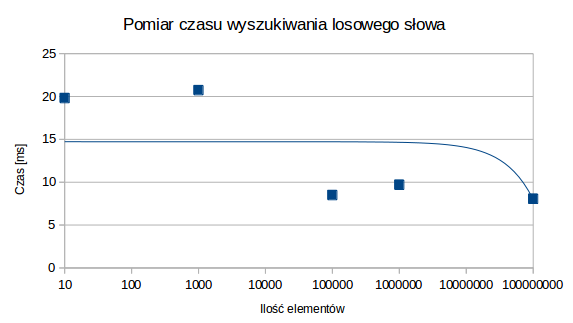
\includegraphics[scale=0.7]{../wyniki/wykres.png}
\end{center}
\end{figure}


\section{Wnioski}
\hspace{4ex}Wyraźnie widać po wynikach pomiarów, że dostęp do każdego elementu jest błyskawiczny.
\end{document}